Ben Trout

2014-10-31

Building Intake, CAD

\begin{tabular}{|p{5cm}|p{5cm}|}
\hline
 Building Intake&
Me and Nick with the help of some other team members were in charge of starting the robot. While I worked on CREO last week Nick finished the base of the robot. Our basic idea is  that This week as building really started to get under way Nick asked if I could help. Me and Nick finished putting on all the wheels and while I attached the intake Nick wired all the wheels and intake motor. we used a cardboard piece that we slit into a curve. We then attached another motor to the very front of our robot and screwed a TETRIX bar to it. Finally, we tapped our cardboard piece on the the bar. By the end of the week we were able to get a driving robot with a rotating intake that can capture balls as it drives around. 
\\
\hline
 CAD&
Me and Filip are still working on CREO to have a virtual robot. Will came down to help us again. He set us up a folder in Windchill and made us our own personal workspaces in Windchill. We can now work on the same robot from different computers and log into our workspaces from any computer. Filip can start a piece and check that piece into Windchill and then I can checkout that piece and start editing the same piece Filip was working on earlier. Me and Filip downloaded all the TETRIX pieces and using the assembly tool in CREO we will start assembling the robot. As we go we can also CAD up different pieces like the ball holder and use the 3D printer to print that piece. 
\\
\hline
\end{tabular}

\section*{Building Intake}
The intake went well for just being a prototype. Our basic idea is reliable and we will probably stick with it. The only problem so far is we need a support on the other side since we’re only using one motor. We also want to put it as far forward on our robot as to not interfere with any of our mechanisms such as the ball launcher. The only problem we had on the actual mechanism is the cardboard over time didn’t have as much of a curve as it lost its rigidity. We’ll definitely be using a 3D piece on our final robot. 


\begin{center}
%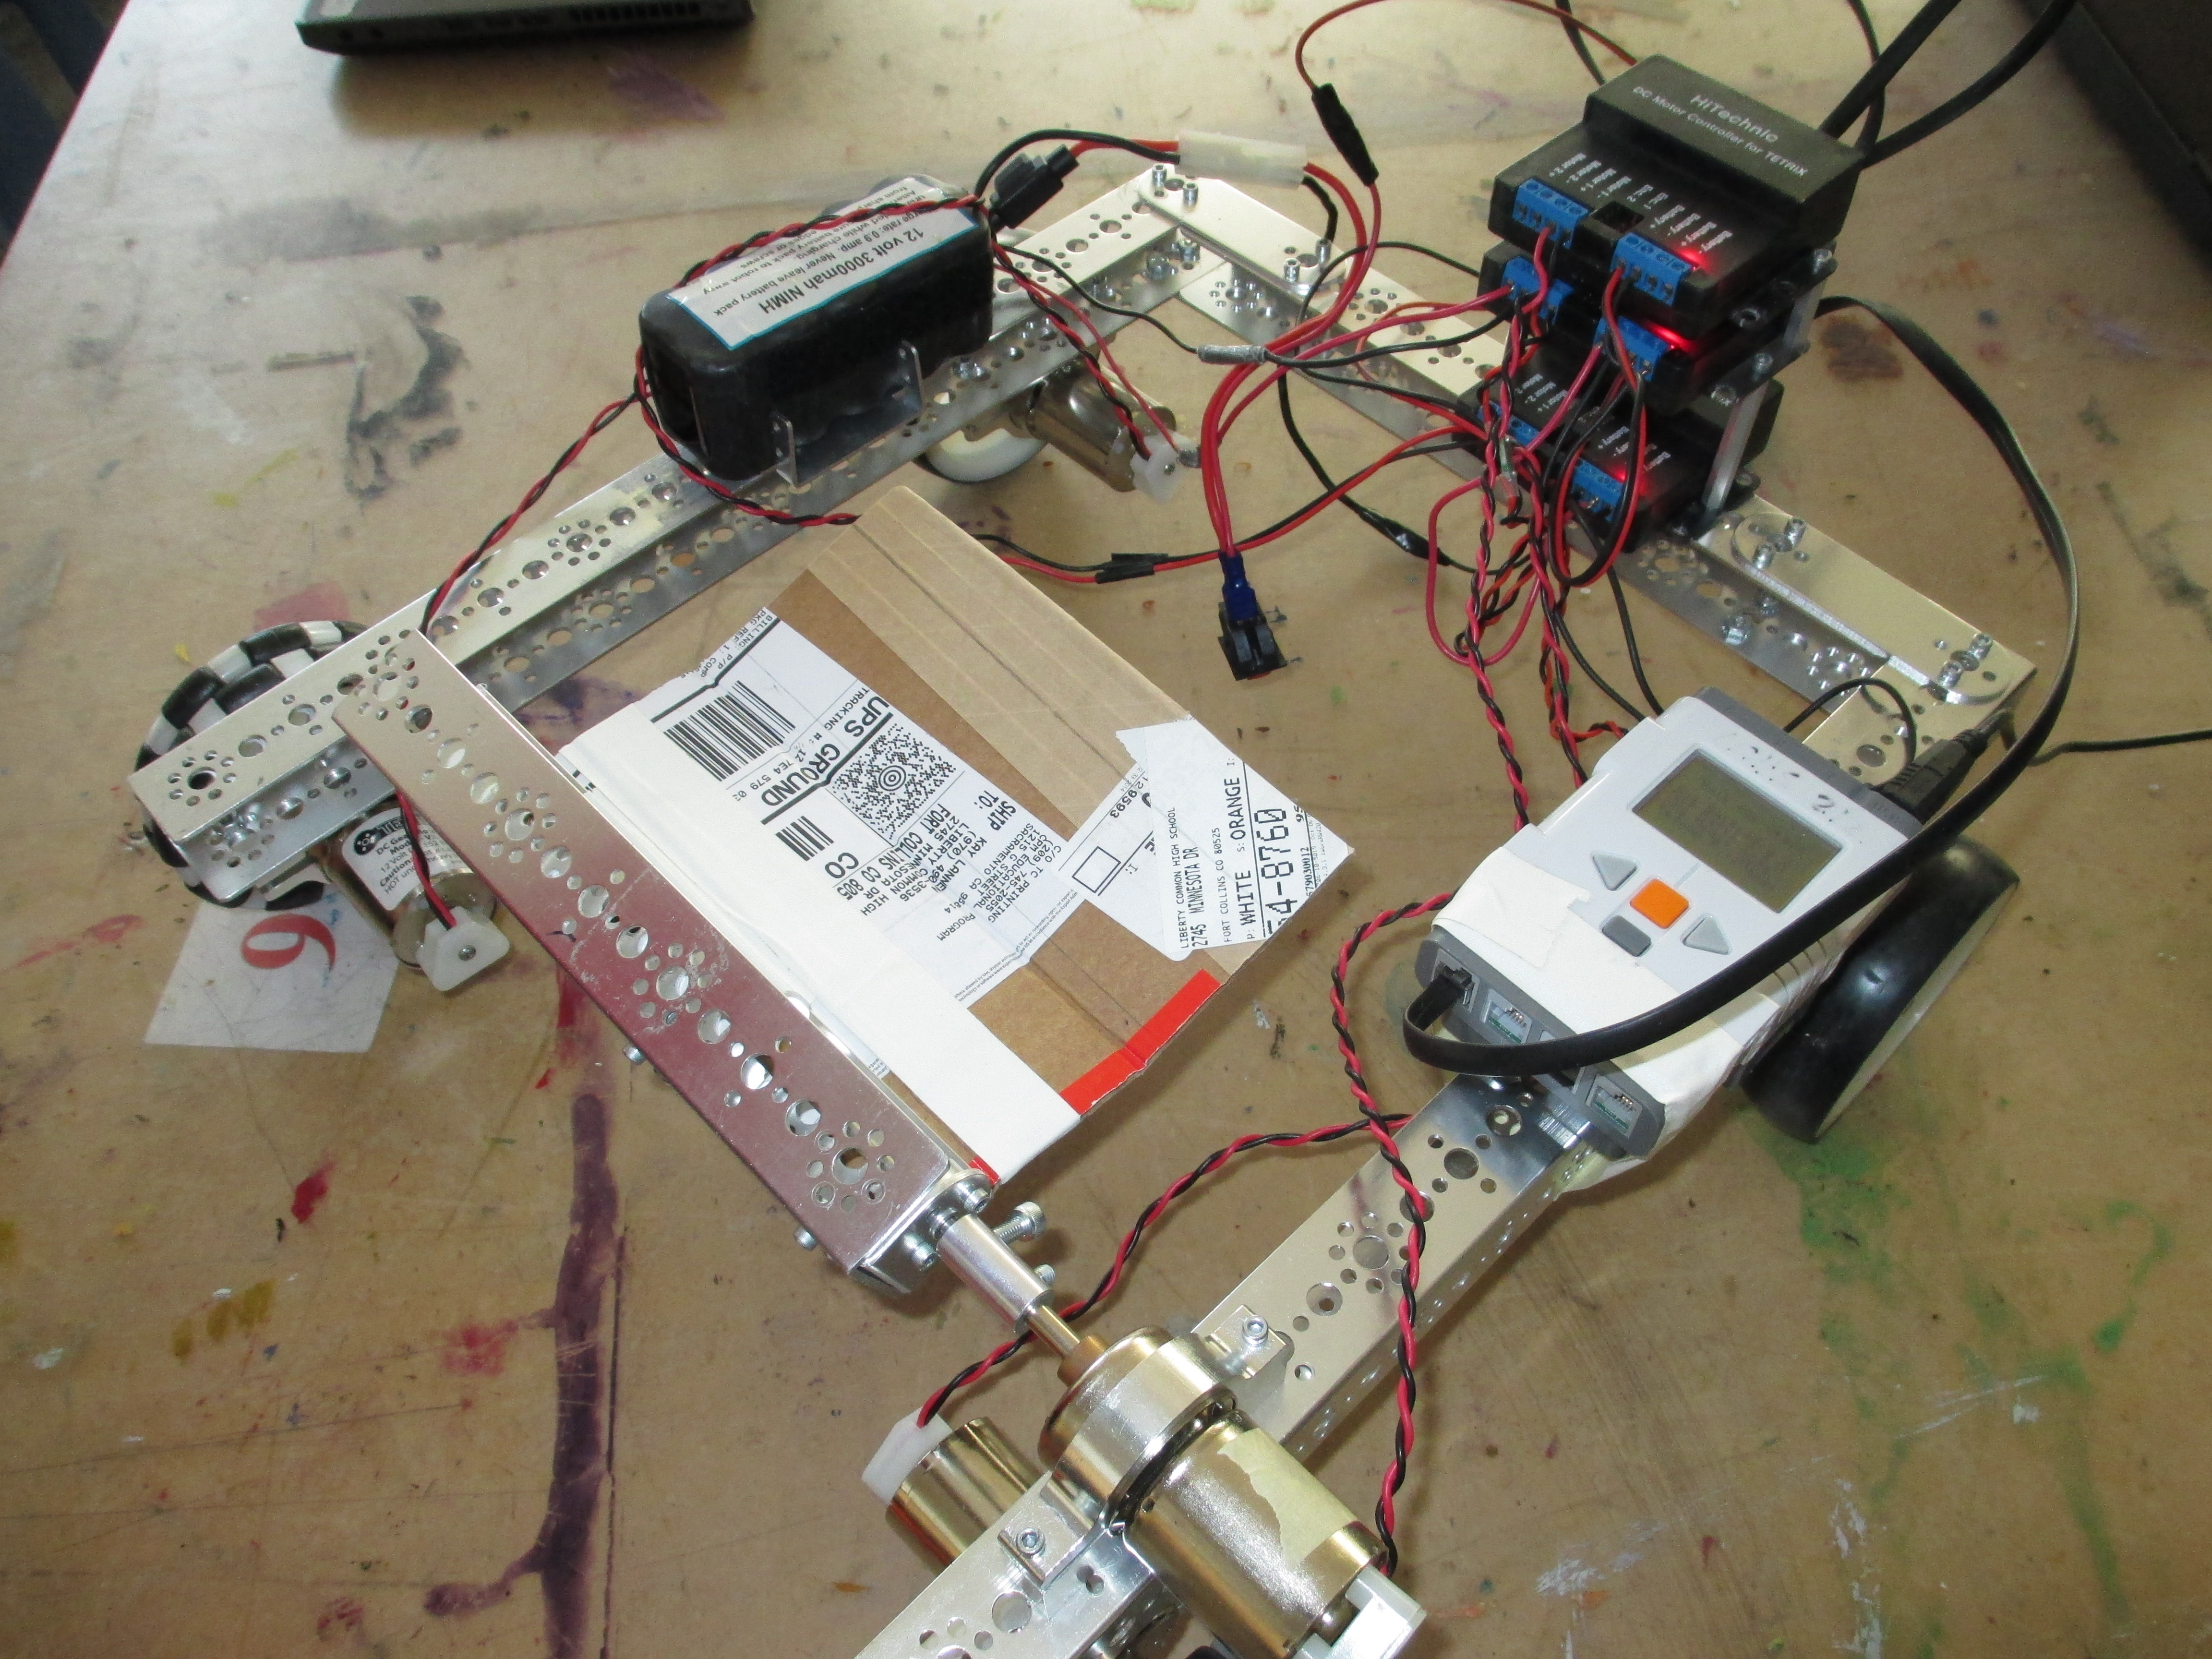
\includegraphics[width=10cm]{./Entries/Images/FirstRotatingBrushProto.jpg} %TODO: Add graphic
\end{center}

The first prototype of our rotating brush in the front of the robot. 